%%
%% 2019 11 14 Ph. G. Freimann
%%

\subsection{Gleichungen mit CAS lösen (optional)}\index{CAS@Computer Algebra System}\index{Computer Algebra System@CAS}
Damit weniger Fehler geschehen, aber auch, um schneller an Resultate zu gelangen werden in der Praxis Gleichungen fast ausschließlich mit einem Computer-Algebra-System (CAS) gelöst.
Wir wählen eine einfache Gleichung, damit wir a) nicht viel tippen müssen und b) das Resultat auch sofort überprüfen können. Gegeben ist also die folgende Gleichung:

$$3x+1=2x$$

Typischerweise bieten sich die folgenden drei Lösungswege an\footnote{Die drei Verfahren wurden mit dem Rechner ``TI-nspire II-CX CAS'' getestet.}:
\begin{itemize}
\item solve($3x+1=2x$, $x$)
\item $\text{gl1} := 3x+1=2x$\\
  solve($\text{gl1}$, $x$)
  
\item $\text{term1} := 3x+1$\\
  $\text{term2} := 2x$\\
  solve($\text{term1}=\text{term2}$, $x$)\\
  Diese letzte Variante hat den Vorteil, dass wir die Terme leicht als Funktionen in $x$ auffassen können und diese im Graph-Modus sofort anzeigen können:
  \begin{enumerate}
    \item Neue «Page» (1.2) erstellen (+page) als Graph. 
    \item Tippe $f1(x)=\text{term1}$
    \item Tippe \fbox{CTRL} \fbox{G} (oder mehrmals die \fbox{TAB}-Taste), um die Eingabezeile wieder zu aktivieren.
      \item $f2(x)=\text{term2}$
  \end{enumerate}

\bbwCenterGraphic{6cm}{tals/gl1/img/nspire_zwei_gleichungen.png}
%  \begin{center}
%   \raisebox{-1cm}{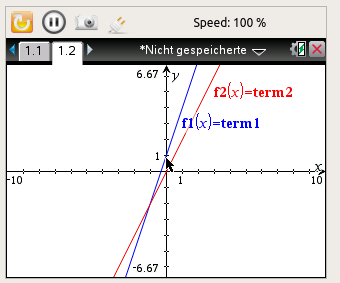
\includegraphics[width=6cm]{img/nspire_zwei_gleichungen.png}}
%  \end{center}
  Der Schnittpunkt der beiden Geraden zeigt die Variable $x$ (hier $-1$) und den Wert der beiden Terme (links bzw. rechts) des Gleichheitszeichens als Variable $y$ (hier $-2$) an.

\end{itemize}

\newpage
